%===============================================================================
% LaTeX sjabloon voor de bachelorproef toegepaste informatica aan HOGENT
% Meer info op https://github.com/HoGentTIN/latex-hogent-report
%===============================================================================

\documentclass[dutch,dit,thesis]{hogentreport}

% TODO:
% - If necessary, replace the option `dit`' with your own department!
%   Valid entries are dbo, dbt, dgz, dit, dlo, dog, dsa, soa
% - If you write your thesis in English (remark: only possible after getting
%   explicit approval!), remove the option "dutch," or replace with "english".

\usepackage{lipsum} % For blind text, can be removed after adding actual content

%% Pictures to include in the text can be put in the graphics/ folder
\graphicspath{{../graphics/}}

%% For source code highlighting, requires pygments to be installed
%% Compile with the -shell-escape flag!
\usepackage[chapter]{minted}
%% If you compile with the make_thesis.{bat,sh} script, use the following
%% import instead:
%%\usepackage[chapter,outputdir=../output]{minted}
\usemintedstyle{solarized-light}

%% Formatting for minted environments.
\setminted{%
    autogobble,
    frame=lines,
    breaklines,
    linenos,
    tabsize=4
}

%% Ensure the list of listings is in the table of contents
\renewcommand\listoflistingscaption{%
    \IfLanguageName{dutch}{Lijst van codefragmenten}{List of listings}
}
\renewcommand\listingscaption{%
    \IfLanguageName{dutch}{Codefragment}{Listing}
}
\renewcommand*\listoflistings{%
    \cleardoublepage\phantomsection\addcontentsline{toc}{chapter}{\listoflistingscaption}%
    \listof{listing}{\listoflistingscaption}%
}

% Other packages not already included can be imported here
\usepackage[toc,acronym]{glossaries}
\makeglossaries{}

%%---------- Document metadata -------------------------------------------------
% TODO: Replace this with your own information
\author{Daniel Boustani}
\supervisor{Dhr. B. Van Vreckem}
\cosupervisor{Dhr. B. Van Vreckem}
\title[]%
    {Eureka: een virtuele assistent dat studenten en docenten bijstaat bij het beantwoorden van vak-gerelateerde vragen}
\academicyear{\advance\year by -1 \the\year--\advance\year by 1 \the\year}
\examperiod{1}
\degreesought{\IfLanguageName{dutch}{Professionele bachelor in de toegepaste informatica}{Bachelor of applied computer science}}
\partialthesis{false} %% To display 'in partial fulfilment'
%\institution{Internshipcompany BVBA.}

%% Add global exceptions to the hyphenation here
\hyphenation{back-slash}

%% The bibliography (style and settings are  found in hogentthesis.cls)
\addbibresource{bachproef.bib}            %% Bibliography file
\addbibresource{../voorstel/voorstel.bib} %% Bibliography research proposal
\defbibheading{bibempty}{}

%% Prevent empty pages for right-handed chapter starts in twoside mode
\renewcommand{\cleardoublepage}{\clearpage}

\renewcommand{\arraystretch}{1.2}

%% Content starts here.
\begin{document}

%---------- Front matter -------------------------------------------------------

\frontmatter

\hypersetup{pageanchor=false} %% Disable page numbering references
%% Render a Dutch outer title page if the main language is English
\IfLanguageName{english}{%
    %% If necessary, information can be changed here
    \degreesought{Professionele Bachelor toegepaste informatica}%
    \begin{otherlanguage}{dutch}%
       \maketitle%
    \end{otherlanguage}%
}{}

%% Generates title page content
\maketitle
\hypersetup{pageanchor=true}

%%=============================================================================
%% Voorwoord
%%=============================================================================

\chapter*{\IfLanguageName{dutch}{Woord vooraf}{Preface}}%
\label{ch:voorwoord}

%% TODO:
%% Het voorwoord is het enige deel van de bachelorproef waar je vanuit je
%% eigen standpunt (``ik-vorm'') mag schrijven. Je kan hier bv. motiveren
%% waarom jij het onderwerp wil bespreken.
%% Vergeet ook niet te bedanken wie je geholpen/gesteund/... heeft

\lipsum[1-2]
%%=============================================================================
%% Samenvatting
%%=============================================================================

% TODO: De "abstract" of samenvatting is een kernachtige (~ 1 blz. voor een
% thesis) synthese van het document.
%
% Een goede abstract biedt een kernachtig antwoord op volgende vragen:
%
% 1. Waarover gaat de bachelorproef?
% 2. Waarom heb je er over geschreven?
% 3. Hoe heb je het onderzoek uitgevoerd?
% 4. Wat waren de resultaten? Wat blijkt uit je onderzoek?
% 5. Wat betekenen je resultaten? Wat is de relevantie voor het werkveld?
%
% Daarom bestaat een abstract uit volgende componenten:
%
% - inleiding + kaderen thema
% - probleemstelling
% - (centrale) onderzoeksvraag
% - onderzoeksdoelstelling
% - methodologie
% - resultaten (beperk tot de belangrijkste, relevant voor de onderzoeksvraag)
% - conclusies, aanbevelingen, beperkingen
%
% LET OP! Een samenvatting is GEEN voorwoord!

%%---------- Nederlandse samenvatting -----------------------------------------
%
% TODO: Als je je bachelorproef in het Engels schrijft, moet je eerst een
% Nederlandse samenvatting invoegen. Haal daarvoor onderstaande code uit
% commentaar.
% Wie zijn bachelorproef in het Nederlands schrijft, kan dit negeren, de inhoud
% wordt niet in het document ingevoegd.

\IfLanguageName{english}{%
\selectlanguage{dutch}
\chapter*{Samenvatting}
\lipsum[1-4]
\selectlanguage{english}
}{}

%%---------- Samenvatting -----------------------------------------------------
% De samenvatting in de hoofdtaal van het document

\chapter*{\IfLanguageName{dutch}{Samenvatting}{Abstract}}

Tijdens hun opleiding aan HOGENT worden studenten geconfronteerd met een grote hoeveelheid informatie over vakken, lesmodaliteiten, deadlines en softwarevereisten. Ondanks de beschikbaarheid van studiemateriaal en andere informatiebronnen blijven er vaak vragen onbeantwoord. Studenten wenden zich eerst tot medestudenten op sociale media om antwoorden te vinden, maar dit kan resulteren tot foutieve of tegenstrijdige informatie. Wanneer ze alsnog geen duidelijk antwoord krijgen, nemen ze contact op met de docent. Dit leidt tot een verhoogde werkdruk en een inefficiënt informatie-uitwisselingsproces.

Deze bachelorproef onderzoekt de haalbaarheid en toepasbaarheid van Eureka, een virtuele assistent die gebruikmaakt van Large Language Models (LLM’s) om studenten en docenten te ondersteunen bij vakgerelateerde vragen. Eureka moet niet alleen correcte en relevante antwoorden genereren, maar ook bronnen vermelden en hallucinaties vermijden. Bovendien moet het systeem robuust zijn tegen ongewenste interacties en eenvoudig uitbreidbaar, zodat ook docenten zonder expertise in LLM-technologie het kunnen gebruiken.

Aangezien het ontwikkelen of volledig fine-tunen van een LLM te veel middelen vereist, wordt gekozen voor Retrieval-Augmented Generation (RAG). Deze techniek combineert een LLM met een externe databank waarin cursusmateriaal wordt opgeslagen. Wanneer een student een vraag stelt, haalt Eureka de relevante informatie op uit de databank en gebruikt deze als context om een accuraat antwoord te genereren. Hierdoor kan het systeem goed functioneren binnen de dynamische onderwijsomgeving, waarin vakinhoud en leermaterialen regelmatig veranderen.

Om Eureka te evalueren, wordt een Proof-of-Concept (PoC) ontwikkeld en getest met vakken gegeven door dhr. Van Vreckem. Dit PoC wordt lokaal opgezet en wordt gezocht naar de ideale LLM, embedder en chunking-techniek combinatie. De PoC wordt geëvalueerd door de gegenereerde antwoorden te laten beoordelen door zowel een vertegenwoordiger van de docenten als een vertegenwoordiger van de studenten. De evaluatiecriteria zijn relevantie, correctheid, bronvermelding en afwezigheid van hallucinaties.

Indien succesvol, wordt Eureka uitgerold op een server en toegankelijk gemaakt via een REST API. Dit onderzoek toont aan dat een LLM-gebaseerde chatbot in combinatie met RAG een efficiënte oplossing kan bieden voor de informatievoorziening binnen HOGENT, waarbij studenten direct toegang krijgen tot betrouwbare antwoorden en de werkdruk van docenten wordt verminderd.

%---------- Inhoud, lijst figuren, ... -----------------------------------------

\tableofcontents

% In a list of figures, the complete caption will be included. To prevent this,
% ALWAYS add a short description in the caption!
%
%  \caption[short description]{elaborate description}
%
% If you do, only the short description will be used in the list of figures

\listoffigures

% If you included tables and/or source code listings, uncomment the appropriate
% lines.
%\listoftables

%\listoflistings

% Als je een lijst van afkortingen of termen wil toevoegen, dan hoort die
% hier thuis. Gebruik bijvoorbeeld de ``glossaries'' package.
% https://www.overleaf.com/learn/latex/Glossaries

\newacronym{AI}{AI}{Artificiële intelligentie}
\newacronym{NLP}{NLP}{Natural Language Processing}
\newacronym{LLM}{LLM}{Large Language Models}
\newacronym{RAG}{RAG}{Retrieval-augmented-generation}
\newacronym{LoRA}{LoRA}{Low-Rank Adaptation}

\newglossaryentry{recommender}
{
    name=Aanbevelingssysteem,
    description={Een algoritme/software die bepaalde items aan gebruikers zal aanbevelen op basis van hun voorkeuren en gedrag. Dergelijke systemen zorgen voor een gepersonaliseerde ervaringen}
}

\newglossaryentry{ChatGPT}
{
    name=ChatGPT,
    description={Een model ontwikkeld door het bedrijf OpenAI dat in staat is om mensachtige interacties te voeren. Met andere woorden, het kan tekst begrijpen en genereren. Dit model kreeg wereldwijd aandacht eind 2022}
}

\newglossaryentry{label}
{
    name=Gelabelde data,
    description={Trainingsdata waarbij elk gegeven voorzien is van een bijbehorende annotatie. Dit annotatie helpt een model patronen te herkennen en correcte voorspellingen te maken. Voorbeeld: indien we een model willen trainen om katten op foto's te herkennen, worden afbeeldingen van katten gelabeld als ``kat''. Hierdoor leert het model onderscheid te maken tussen katten en andere objecten}
}

\printglossary{}
\printglossary[type=\acronymtype]

%---------- Kern ---------------------------------------------------------------

\mainmatter{}

% De eerste hoofdstukken van een bachelorproef zijn meestal een inleiding op
% het onderwerp, literatuurstudie en verantwoording methodologie.
% Aarzel niet om een meer beschrijvende titel aan deze hoofdstukken te geven of
% om bijvoorbeeld de inleiding en/of stand van zaken over meerdere hoofdstukken
% te verspreiden!

%%=============================================================================
%% Inleiding
%%=============================================================================

\chapter{\IfLanguageName{dutch}{Inleiding}{Introduction}}%
\label{ch:inleiding}

%De inleiding moet de lezer net genoeg informatie verschaffen om het onderwerp te begrijpen en in te zien waarom de onderzoeksvraag de moeite waard is om te onderzoeken. In de inleiding ga je literatuurverwijzingen beperken, zodat de tekst vlot leesbaar blijft. Je kan de inleiding verder onderverdelen in secties als dit de tekst verduidelijkt. Zaken die aan bod kunnen komen in de inleiding~\autocite{Pollefliet2011}:
%
%\begin{itemize}
%  \item context, achtergrond
%  \item afbakenen van het onderwerp
%  \item verantwoording van het onderwerp, methodologie
%  \item probleemstelling
%  \item onderzoeksdoelstelling
%  \item onderzoeksvraag
%  \item \ldots
%\end{itemize}

\section{\IfLanguageName{dutch}{Probleemstelling}{Problem Statement}}%
\label{sec:probleemstelling}

%Uit je probleemstelling moet duidelijk zijn dat je onderzoek een meerwaarde heeft voor een concrete doelgroep. De doelgroep moet goed gedefinieerd en afgelijnd zijn. Doelgroepen als ``bedrijven,'' ``KMO's'', systeembeheerders, enz.~zijn nog te vaag. Als je een lijstje kan maken van de personen/organisaties die een meerwaarde zullen vinden in deze bachelorproef (dit is eigenlijk je steekproefkader), dan is dat een indicatie dat de doelgroep goed gedefinieerd is. Dit kan een enkel bedrijf zijn of zelfs één persoon (je co-promotor/opdrachtgever).

Bij het opnemen van een vak worden studenten aan de HOGENT tijdens het semester vaak geconfronteerd met een grote hoeveelheid informatie: lesmodaliteiten, taken, deadlines, en kennismaking met de benodigde software, om enkele voorbeelden te noemen. Gedurende het semester ontstaan er regelmatig vragen bij studenten, die zij proberen te beantwoorden door de beschikbare materialen te raadplegen of door hun vragen aan medestudenten voor te leggen. Toch blijken deze informatiebronnen niet altijd voldoende --- vanwege onduidelijkheden of tegenstrijdigheden --- zoals blijkt uit het aantal studenten dat alsnog bij de docent aanklopt. Dit is echter niet praktisch; als een docent tien keer dezelfde vraag ontvangt, moet hij of zij die vraag ook tien keer beantwoorden. Bovendien is er geen garantie dat een student zijn of haar antwoord dezelfde dag nog ontvangt. Deze uitwisseling is dan ook een frustrerend en tijdrovend proces voor beide partijen. Er bestaat dus behoefte aan een middel dat enerzijds de werkdruk van docenten verlicht door antwoorden te geven op veelgestelde vragen van studenten en anderzijds deze antwoorden on demand levert. 

\section{\IfLanguageName{dutch}{Onderzoeksvraag}{Research question}}%
\label{sec:onderzoeksvraag}

%Wees zo concreet mogelijk bij het formuleren van je onderzoeksvraag. Een onderzoeksvraag is trouwens iets waar nog niemand op dit moment een antwoord heeft (voor zover je kan nagaan). Het opzoeken van bestaande informatie (bv. ``welke tools bestaan er voor deze toepassing?'') is dus geen onderzoeksvraag. Je kan de onderzoeksvraag verder specifiëren in deelvragen. Bv.~als je onderzoek gaat over performantiemetingen, dan 

Dankzij de technologische vooruitgang van de afgelopen jaren staat het vakgebied van \acrfull{AI} opnieuw in de schijnwerpers. \acrlong{AI} blijkt een krachtige tool te zijn voor het oplossen van complexe problemen die voor mensen moeilijk of zelfs onmogelijk op te lossen zijn. Zo wordt \acrshort{AI} ingezet om de \gls{recommender} van Netflix te verbeteren \autocite{Steck2021}, voor de vroege detectie van aandoeningen zoals Alzheimer \autocite{Lewis2024}, en om het werk van fastfoodmedewerkers te verlichten door bestellingen bij drive-thrus automatisch op te nemen \autocite{Kinnear2024}, om er maar enkele te noemen.

Tussen al deze toepassingen is er één die onze aandacht meer dan de andere heeft getrokken, namelijk \acrfull{LLM} (zie~\ref{sec:llms}). \acrshort{LLM}'s zijn modellen die in staat zijn menselijke taal te begrijpen en te genereren. De beroemdste van hen is zonder twijfel \emph{\gls{ChatGPT}}. Dit model heeft de wereld stormenderhand veroverd dankzij zijn vermogen om mensachtige gesprekken te voeren en de verscheidenheid aan taken die het kan uitvoeren. Deze revolutie heeft geleid tot de geboorte van een nieuwe generatie chatbot die gebruikmaken van \acrshort{LLM}'s als onderliggende technologie (zie~\ref{sec:chatbots}). In onze zoektocht naar een oplossing voor het bovengenoemde probleem lijken dergelijke chatbots een mogelijke uitkomst te bieden.

In deze bachelorproef wordt de haalbaarheid van Eureka, een virtuele assistent die studenten en docenten ondersteunt bij het beantwoorden van vakgerelateerde vragen, en de toepasbaarheid ervan binnen de context van HOGENT onderzocht. Met andere woorden, we willen achterhalen of een dergelijke chatbot een geschikte oplossing biedt voor het voorliggende probleem en in welke mate deze effectief is.
 
\section{\IfLanguageName{dutch}{Onderzoeksdoelstelling}{Research objective}}%
\label{sec:onderzoeksdoelstelling}

%Wat is het beoogde resultaat van je bachelorproef? Wat zijn de criteria voor succes? Beschrijf die zo concreet mogelijk. Gaat het bv.\ om een proof-of-concept, een prototype, een verslag met aanbevelingen, een vergelijkende studie, enz.

De haalbaarheid en toepasbaarheid van Eureka worden getoetst aan de hand van een \emph{Proof-of-Concept} (PoC). Deze PoC moet aan bepaalde criteria voldoen, zowel vanuit het probleemdomein als het oplossingsdomein, om als succesvol te worden beschouwd. Deze criteria vloeien voort uit de verwachtingen die studenten en docenten hebben van een dergelijke tool.

Betreffende het probleemdomein wordt verwacht dat Eureka relevante antwoorden genereert; dit is immers de bestaansreden van deze tool. De bron van het antwoord moet ook worden meegedeeld, zodat de student of docent de betrouwbaarheid van de informatie kan verifiëren en deze verder kan doorzoeken indien gewenst. Daarnaast wordt verwacht dat hallucinaties (zie~\ref{subsec:valkuilen}) strikt worden vermeden. Als valse informatie wordt verspreid, leidt dit tot meer verwarring en werkt het tegen het nut van deze tool in.

Ten slotte wordt ook verwacht dat Eureka onverwachte interacties, zoals beledigingen, aankan. De menselijke natuur is onvoorspelbaar en dergelijke interacties zullen zich voordoen. Eureka moet hier robuust tegen zijn.

Voor het oplossingsdomein wordt verwacht dat Eureka op een eenvoudige manier kan worden uitgebreid of gewijzigd. De schoolomgeving is zeer dynamisch en wijzigingen komen regelmatig voor. Deze wijzigingen moeten snel kunnen worden doorgevoerd in Eureka en op een gebruiksvriendelijke manier, zodat ook docenten zonder gespecialiseerde technische kennis of expertise in het vakgebied dit kunnen doen.

Bovendien moet de toepassing van Eureka rekening houden met de beperkte financiële en computationele middelen waarover we beschikken.

\section{\IfLanguageName{dutch}{Opzet van deze bachelorproef}{Structure of this bachelor thesis}}%
\label{sec:opzet-bachelorproef}

% Het is gebruikelijk aan het einde van de inleiding een overzicht te
% geven van de opbouw van de rest van de tekst. Deze sectie bevat al een aanzet
% die je kan aanvullen/aanpassen in functie van je eigen tekst.

De rest van deze bachelorproef is als volgt opgebouwd:

In Hoofdstuk~\ref{ch:literatuurstudie} bekijken we eerst de huidige situatie binnen HOGENT. We analyseren de verschillende informatiebronnen die studenten ter beschikking hebben en hoe deze de docenten beïnvloeden. Vervolgens onderzoeken we de stand van zaken binnen het onderzoeksdomein op basis van een literatuurstudie. Hierin geven we een kort overzicht van de geschiedenis van chatbots en zien we dat de huidige generatie chatbots gebaseerd is op \acrshort{LLM}'s. Daarna bespreken we wat \acrshort{LLM}'s zijn.

Aangezien we een chatbot willen ontwerpen voor een specifieke use-case binnen HOGENT, bekijken we in de twee volgende onderdelen hoe een \acrshort{LLM} gespecialiseerd kan worden en wat er allemaal komt kijken bij de gekozen techniek. Uiteindelijk sluiten we de literatuurstudie af door de mogelijke valkuilen te benoemen die kunnen optreden bij het implementeren van dergelijke technologie.

In Hoofdstuk~\ref{ch:methodologie} wordt de methodologie toegelicht. Hier bespreken we hoe het onderzoek is opgedeeld. Het onderzoek bestaat uit een ontdekkingsfase, een implementatiefase en een testfase.

De ontdekkingsfase heeft als doel een \acrshort{LLM} te vinden die aan bepaalde verwachtingen voldoet. Deze fase wordt uitgevoerd in een beperkte en gecontroleerde omgeving.

De implementatiefase omvat de daadwerkelijke implementatie van Eureka. Hierbij wordt een pijplijn opgebouwd, samengesteld uit verschillende componenten. Elk van deze componenten en hun functie worden verder toegelicht.

Tijdens de testfase wordt Eureka geëvalueerd aan de hand van de gestelde verwachtingen. Hiervoor worden persona's gebruikt.

Bij elke fase wordt ook een ingeschatte duurtijd vermeld.

% TODO: Vul hier aan voor je eigen hoofstukken, één of twee zinnen per hoofdstuk

In Hoofdstuk~\ref{ch:conclusie}, tenslotte, wordt de conclusie gegeven en een antwoord geformuleerd op de onderzoeksvragen. Daarbij wordt ook een aanzet gegeven voor toekomstig onderzoek binnen dit domein.
\chapter{\IfLanguageName{dutch}{Literatuurstudie}{Literature review}}%
\label{ch:literatuurstudie}

\section{\IfLanguageName{dutch}{Stand van zaken}{State of the art}}%
\label{sec:state-of-the-art}

Om informatie te verkrijgen, onderscheiden veel studenten twee belangrijke informatiebronnen: bronnen afkomstig van de hogeschool en informatie uitgewisseld door studenten zelf.

Vanuit de hogeschool worden verschillende informatiebronnen aangeboden waarop studenten en docenten antwoorden kunnen vinden op hun vragen. Ten eerste zijn er de inleidende slides van het vak. Hierin is informatie te vinden over eventueel aan te schaffen materialen, mogelijke softwarevereisten, deadlines en de organisatie van het vak. Naast de inleidende slides zijn er de gewone slides, die de vakinhoud bevatten. Verder zijn er de studiefiches, waarin algemene informatie staat zoals de studielast, de leerresultaten en de evaluatievorm. Bij sommige vakken worden ook aanvullende bestanden verstrekt die studenten begeleiden bij bepaalde onderwerpen en vaak voorkomende problemen of vragen behandelen. Tot slot is bij sommige vakken ook een forum beschikbaar. Dit forum dient als centrale plaats om vragen te stellen, waarbij de antwoorden zichtbaar zijn voor alle studenten.

Daarnaast maken veel mensen gebruik van sociale media om informatie over specifieke onderwerpen uit te wisselen, en studenten vormen hierop geen uitzondering. Sociale media wordt ingezet om met andere studenten over de vakinhoud te communiceren en zo nieuwe kennis op te doen. Deze veronderstelling is ook bevestigd in andere onderzoeken. \textcite{M.Talaue2018} en \textcite{Bal2017} interviewden verschillende studenten over hun gebruik van sociale media, waaruit blijkt dat een groot deel van hen sociale media gebruikt om vakken hun inhoud te bespreken. Aan de HOGENT is dit eveneens het geval. Naast hun persoonlijke profielen op andere media, komen studenten samen op een \textit{Discord}-server. Deze server is onderverdeeld in verschillende kanalen, waarbij elk kanaal een specifiek vak vertegenwoordigt. Studenten bespreken in deze kanalen alles wat met het desbetreffende vak te maken heeft en stellen er hun vragen. Aangezien deze server door studenten wordt beheerd en docenten er geen toegang toe hebben, omdat het \textbf{geen officieel kanaal van HOGENT} is, bestaat het risico dat er foutieve informatie wordt uitgewisseld. 

Zoals blijkt, is informatie verspreid over een verscheidenheid aan media. Informatie vinden kan daarom enige moeite kosten, en de kans op onduidelijkheden of tegenstrijdige informatie is aanzienlijk. In het geval van problemen is het laatste redmiddel voor studenten om contact op te nemen met de docent. De positie van docenten stelt hen in staat om onduidelijkheid op te helderen, maar zij beschikken niet altijd over de tijd hiervoor. Bovendien kan het herhaaldelijk beantwoorden van dezelfde vragen frustrerend zijn.

We concluderen daarom dat er behoefte is aan een middel dat het zoekproces intuïtiever maakt en de belasting voor alle betrokken partijen verlicht. Wij stellen hiervoor een chatbot in de vorm van een virtuele assistent voor en zullen deze oplossing verder onderzoeken.

\section{\IfLanguageName{dutch}{Evolutie van chatbots}{Evolution of chatbots}}%
\label{sec:chatbots}

In de jaren zestig begon men met de eerste onderzoeken naar communicatie tussen computers en mensen. De onderzoekers hadden niet de intentie om grote doorbraken in het veld te realiseren, maar wilden enkel experimenteren met de grens tussen mens en machine \autocite{Dibitonto2018, AbuShawar2007}. Een van deze experimenten was \textit{ELIZA} \autocite{Weizenbaum1966}. ELIZA was ''een computerprogramma [...] dat bepaalde natuurlijke taalgesprekken tussen mens en computer mogelijk maakte''. Het werd ontwikkeld voor de IBM 7094 en geschreven in MAD-SLIP \autocite{Weizenbaum1966}. De werking van ELIZA kan grofweg als volgt worden samengevat: gegeven een invoerzin, werden vooraf gedefinieerde sleutelwoorden gezocht. Eens deze sleutelwoorden gevonden werden, werd het uiteindelijke antwoord gegenereerd door gebruik te maken van reconstructieregels. 

Naargelang de onderzoek naar chatbots vorderde, werden betere architecturen bedacht maar de kern bleef onveranderd: pattern-matching-algortimen die regels toepasten met als doel de interactie zo natuurlijk mogelijk te laten aanvoelen \autocite{AbuShawar2007}. Hoewel de toepassing van chatbots als virtuele assistenten of informatieopzoeksystemen destijds als succesvol werd beschouwd \autocite{AbuShawar2007}, is het niet moeilijk voor te stellen hoe vatbaar deze technologie is voor fouten en rigiditeit. Wanneer een bepaalde casus niet wordt gedekt door een regel of de regels onvoldoende doordacht zijn, presteert de chatbot slecht, waardoor de interactie wordt belemmerd. 

Dankzij de toenemende rekenkracht van de afgelopen jaren en de groeiende interesse in het domein van artificiële intelligentie, zien we een nieuwe generatie chatbots ontstaan. De werking van deze chatbots maakt het mogelijk om af te stappen van het pattern-matching-paradigma. Deze chatbots maken namelijk gebruik van doorbraken in \acrfull{NLP} en zijn gebaseerd op \arcfull{LLM} (zie \ref{sec:llms}). Dergelijke chatbots worden al in verschillende domeinen gebruikt met overtuigende resultaten \autocite{Dell’Acqua2023, Wang2024, Azam2024}

\section{Large Language Models}%
\label{sec:llms}

Sinds eind 2022 heeft vrijwel iedereen minstens één keer gehoord van \textit{ChatGPT}. Een analyse van de populariteit van deze term via \textit{Google Trends} laat zien dat de interesse in \textit{ChatGPT} voortdurend toeneemt. Een doorbraak in artificiële intelligentie heeft Large Language Models en, in bredere zin, Natural Language Processing in de schijnwerpers gezet. NLP kan worden gedefinieerd als ''de tak van Artificiële Intelligentie die computers helpt menselijke taal te begrijpen, interpreteren en manipuleren'' \autocite{Zohuri2022}. Het omvat een reeks technieken die het mogelijk maken voor computers om op een natuurlijke manier te communiceren met mensen. LLM's daarentegen zijn intelligente systemen die, door gebruik te maken van NLP-technieken, in staat zijn om tekst te verwerken en te genereren met samenhangende communicatie. Hoewel LLM's zeer populair zijn vandaag, is hun werking voor de meerderheid van mensen nog magie. Zodat de lezer een idee kan krijgen van wat er allemaal verbogen staat achter een LLM, geven we hier een bondig samenvatting dat gebaseerd is op \textcite{Naveed2023}.

Eem LLM is een zeer diepe kunstmatige neurale netwerken dat rust op de \textit{transformer} architectuur (geïntroduceerd door \textcite{Vaswani2017}). Elke moderne LLM heeft volgende basiscomponenten: 
\begin{itemize} 
    \item \textbf{Tokenisatie}: Dit is een pre-processing stap dat training voorgaat. Hier, wordt de invoer onderverdeelt in tokens. Een token kan een character, stuk woord, symbool of woord zijn afhankelijk van de tokenisatie-techniek dat gebruikt wordt.
    \item \textbf{Aandacht}: Deze component wijst gewichten toe aan de input tokens zodat de model meer aandacht richt aan de belangrijkste tokens.
    \item \textbf{Positionele encodering}: Hier wordt informatie toegevoegd met betrekking tot de posities van de tokens. Dit component werkt heel nauw samen met de aandacht zodat de model de invoer begrijpt. Anders uitgedrukt, wordt via aandacht de belangrijkste toekens geïdentificieert en via positionele encodering wordt de volgorde en context van deze tokens verstaan.
    \item \textbf{Activatiefunctie}: Deze functies laten toe de model om niet-lineaire relaties aan te leren, wat cruciaal is om met taal aan de slag te gaan.
\end{itemize}

De training van de LLM gebeurt volgens \textcite{Bach2024} in drie fases:
\begin{enumerate} 
    \item \textbf{Self-supervised learning}: In deze stap moet de LLM, gegeven een zin met een ontbrekend woord (of woorden), een lijst genereren van mogelijke woorden die zouden kunnen passen. Deze lijst is gerangschikt op basis van waarschijnlijkheid. Het doel van deze fase is dat het model de eigenschappen van de taal leert begrijpen, evenals de specifieke kenmerken van het datadomein.
    \item \textbf{Supervised learning}: Hier wordt het model getrained om taken uit te voeren. Voorbeelden van dergelijke taken zijn het genereren van code, het samenvatten van teksten en het beantwoorden van specifieke vragen, om er maar enkele te noemen. Het doel van deze fase is ervoor te zorgen dat het model daadwerkelijk nuttige taken kan uitvoeren in plaats van simpelweg woorden te raden.
    \item \textbf{Reinforcement learning}: In deze stap worden de gewenste gedragen aan het model aangeleerd. Dit gebeurt door gewenst gedrag te belonen en ongewenst gedrag te bestraffen.
\end{enumerate}

De indrukwekkende prestaties van LLM's in een reeks van taken (\autocite{Naveed2023}) zijn te danken aan de hedendaagse rekenkracht, de e\-nor\-me hoeveelheid beschikbare data (voortgebracht door sociale media en het \textit{Internet of Things}), en de groeiende interesse in dit domein \autocite{Zohuri2022, Naveed2023}. Hierdoor zijn LLM's uitermate geschikt als basis voor de ontwikkeling van Eureka. 

\section{\IfLanguageName{dutch}{Ontwerp}{Design}}%
\label{sec:ontwerp}

\subsection{\IfLanguageName{dutch}{Specialiseren van LLM's}{Specializing LLM's}}%
\label{subsec:specialiseren_llm}

Het doel van dit onderzoek is om een chatbot te implementeren, gebaseerd op een LLM, die vragen over vakken \textbf{gegeven aan de HOGENT} kan beantwoorden. Dit betekent dat onze LLM gespecialiseerde kennis moet hebben, in plaats van de algemene kennis die door bekende LLM's wordt gebruikt. Om een LLM te specialiseren, zijn er drie benaderingen mogelijk: zelf een LLM ontwerpen, een bestaande LLM \textit{fine-tunen}, of de kennis van een LLM uitbreiden met behulp van \textit{context-injectie}

De eerste benadering houdt in dat we zelf een LLM vanaf nul bouwen en trainen op door ons aangeleverde data. Dit is echter niet haalbaar vanwege de aanzienlijke middelen, expertise \autocite{Naveed2023} en tijd die hiervoor nodig zijn. \textcite{Fourrier2024} somt verschillende open-source LLM's op, waarvan de meeste meer dan één miljard parameters bevatten. Het is duidelijk dat het trainen van een model met één miljard parameters veel tijd kost en dat het ontwikkelen van een dergelijk model ook een hoog niveau van expertise vereist.

Bij de tweede benadering wordt een bestaande LLM gebruikt, waarbij de gewichten worden aangepast om de LLM te specialiseren voor het specifieke doel waarvoor we deze nodig hebben. Zo hebben \textcite{Azam2024} PharmaLLM ontwikkeld, een chatbot die vragen over medicijnen kan beantwoorden. Dit model werd ontworpen door het Llama 2-model te fine-tunen met behulp van \acrfull{LoRA}. Met LoRA worden alleen de meest impactvolle gewichten aangepast om het model te specialiseren, waardoor het niet nodig is om alle gewichten van het model volledig te hertrainen. Enkel een subset van de gewichten wordt gewijzigd, wat aanzienlijk minder middelen vereist dan de eerste benadering. Hierdoor wordt de specialisatie haalbaar zonder de volledige parameterstructuur te hertrainen.

Hoewel de tweede benadering haalbaarder lijkt, blijven de vereiste middelen aanzienlijk. Zo beschrijven \textcite{Chiang2023} de ontwikkeling van een LLM waarbij zij het model hebben gefinetuned. Om aan hun criteria te voldoen, maakten ze gebruik van acht \textit{A100}-GPU's, waarbij elke trainingssessie meer dan 300 dollar kostte. Bovendien is er, om de juiste fine-tuningtechniek te kiezen - LoRA is niet de enige techniek - en het model optimaal te fine-tunen, opniew expertise vereist.

De laatste benadering maakt gebruikt van een techniek die we context-injectie gaan noemen. Elk LLM beschikt over een \textit{contextvenster}. In dit venster kan extra context worden toegevoegd die het LLM in rekening neemt bij het genereren van zijn antwoord. Het doel van context-injectie is om relevante informatie met betrekking tot de gestelde vraag in het venster te plaatsen. De informatie over de vakken wordt opgeslagen in een databank. Afhankelijk van de gestelde vraag halen we alleen de relevante informatie op. Met deze benadering kunnen we een bestaande LLM gebruiken zonder een trainingsfase, wat resulteert in lagere middelen en expertise die gemakkelijker toegankelijk is. Context-injectie samen met de data vanuit een databank ophalen is wat men \acrfull{RAG} noemt. Deze techniek wordt al succesvol toegepast in verschillende domeinen. We nodigen de lezer uit om \textcite{Wang2024} te raadplegen voor een voorbeeld van ee chatbot die gebruikmaakt van RAG en een vergelijkbaar doel nastreeft als het onze. 

De laatste benadering is de meest veelbelovende met betrekking tot onze doelstellingen. Ze vraagt minder middelen en vereist geen vakexpertise om te benutten. We onderzoeken deze piste verder.

\subsection{Retrieval-augmented-generation}%
\label{subsec:rag}

In 2020 maakten \textcite{Lewis2020} de volgende vaststelling: LLM's zijn zeer geschikt om diepe inzichten te verkrijgen uit de data waarop ze getraind zijn. Hierdoor hebben ze geen externe \textit{knowledge bases} nodig om vragen te beantwoorden; hun vergaarde kennis fungeert als een impliciete knowledge base. Echter brengt dit enkele uitdagingen met zich mee. Ten eerste is het moeilijk om bestaande kennis te actualiseren zonder het leerproces volledig opnieuw te starten. Dit vormt een tijdrovend proces wanneer frequente updates noodzakelijk zijn. Daarnaast hebben LLM's moeite om vragen te beantwoorden over gebeurtenissen die zich hebben voorgedaan na hun laatste trainingssessie, aangezien ze deze kennis niet bezitten. Dit kan leiden tot hallucinaties \autocite{Gao2023}.

Om deze beperkingen aan te pakken, introduceerden de auteurs een nieuwe techniek genaamd Retrieval-Augmented Generation (RAG). Bij deze techniek wordt een vraag beantwoord door aanvullende kennis op te halen uit externe bronnen en deze te gebruiken om een antwoord te genereren. Zoals \textcite{Lewis2020} het omschrijven: ''De invoersequentie $x$ wordt gebruikt om tekstdocumenten $z$ op te halen, die vervolgens dienen als aanvullende context bij het genereren van de doelsequentie $y$''.

Alle RAG-systemen bestaan uit drie belangrijke stappen \autocite{Gao2023}:  

\begin{enumerate} 
    \item \textbf{Indexing}: Hier wordt ruwe data uit verschillende formaten (bijvoorbeeld PDF, HTML, DOCX) opgehaald. Vervolgens wordt deze data geconverteerd naar tekst en opgeschoond. Belangrijk hierbij is dat de tekst wordt opgedeeld in brokken. De reden hiervoor is dat het contextvenster van LLM's een beperkte grootte heeft, waardoor het beter is om alleen de relevante brok door te geven in plaats van het gehele document, waarbij het risico bestaat dat niet alles past. Bovendien is uit onderzoek gebleken dat LLM's meer aandacht besteden aan het begin en einde van het contextvenster en minder aan het midden. Dit fenomeen staat bekend als het \textit{lost in the middle}-fenomeen \autocite{Databricks}. Daarom is het beter om kleinere contexten door te geven dan grote, zodat de aandacht van de LLM behouden blijft. Uiteindelijk, worden de brokken opgeslaan in een vector-databank door gebruik te gaan maken van \textit{embedding} encodering.
    \item \textbf{Retrieval}: In deze fase wordt de gebruikersinvoer omgezet in een vectorvoorstelling met behulp van dezelfde encodering als in de vorige stap. Op basis van deze vectorvoorstelling worden de relevante brokken opgehaald. Relevantie in deze context verwijst naar de brokken die een verband hebben met de gestelde vraag. Dit verband wordt bepaald door middel van vectorvergelijkingen. De opgehaalde brokken worden vervolgens gebruikt om het contextvenster te verrijken.
    \item \textbf{Generation}: Tot slot wordt het finale antwoord gegenereerd. Merk op dat de LLM voornamelijk wordt gebruikt voor haar taalcapaciteiten bij het formuleren van het antwoord. Het grootste deel van het werk wordt echter uitgevoerd in de twee voorgaande fases.
\end{enumerate}

\subsection{\IfLanguageName{dutch}{Valkuilen}{Pitfalls}}%
\label{subsec:valkuilen}

Bij het ontwerpen van Eureka zijn er twee belangrijke valkuilen die bijzondere aandacht vereisen: \textbf{onverwachte interacties} en \textbf{hallucinaties}.

Tijdens de ontwikkeling van de chatbot \textit{LiSA} constateerden \textcite{Dibitonto2018} dat er een tendens bestond om LiSA te antropomorfiseren, ondanks haar beperkte complexiteit. Dit resulteerde in onverwachte reacties, zoals uitingen van dankbaarheid of het gebruik van smileys om zinnen te benadrukken. Helaas leidde dit ook tot ongepast gedrag; sommige gebruikers reageerden agressief of gaven de interactie een seksuele connotatie. Onverwachte interacties kunnen echter niet alleen voortkomen uit gebruikers, maar ook uit de chatbot zelf.

Een voorbeeld hiervan is \textit{Prompt Hacking}, een aanvalsmethode waarbij specifieke prompts worden ingevoerd met als doel de LLM gedrag te laten vertonen dat afwijkt van de oorspronkelijke bedoeling van het model \autocite{Rababah2024}. Dergelijk afwijkend gedrag kan bijvoorbeeld bestaan uit het openbaar maken van privé-informatie of het maken van beledigende opmerkingen \autocite{Naveed2023}.

Daarnaast is vastgesteld dat LLM's onderhevig kunnen zijn aan een fenomeen dat bekend staat als \textit{hallucinatie}. Hierbij genereert de LLM coherente uitvoer die echter gebaseerd is op onjuiste informatie. Dit fenomeen kan worden onderverdeeld in drie categorieën \autocite{Naveed2023}:

\begin{itemize} 
    \item \textbf{Input-conflicterende hallucinatie}: de gegenereerde output heeft weinig tot geen verband met de ingevoerde gegevens. 
    \item \textbf{Context-conflicterende hallucinatie}: de gegenereerde output is in tegenspraak met eerder gegenereerde output. 
    \item \textbf{Feit-conflicterende hallucinatie}: de output bevat onjuiste informatie over algemeen bekende feiten (bijvoorbeeld: ''Parijs is de hoofdstad van Pakistan''). 
\end{itemize}

Hallucinaties dienen strikt vermeden te worden bij het ontwerpen van Eureka, aangezien ze het risico met zich meebrengen om meer verwarring te zaaien in plaats van duidelijkheid te bieden.

\section{\IfLanguageName{dutch}{Besluit}{Conclusion}}%
\label{sec:besluit}

Uit de literatuurstudie blijkt dat een chatbot een geschikte oplossing biedt om een centrale plaats te creëren waar studenten en docenten op een interactieve manier hun vragen kunnen stellen en on-demand een antwoord kunnen ontvangen.

Chatbots zijn een technologie die al geruime tijd bestaat en oorspronkelijk voornamelijk gebaseerd was op patroonherkenning. Met de vooruitgang in NLP en, meer specifiek, in LLM's, kunnen we nu flexibelere chatbots ontwikkelen die niet langer afhankelijk zijn van strikt gedefinieerde regels. Het zelf ontwikkelen van een LLM valt echter buiten de scope van dit onderzoek en overschrijdt de beschikbare middelen. Daarom is besloten om een bestaande LLM te gebruiken.

Aangezien bestaande LLM's vaak worden geleverd met vooraf vergaarde kennis, en we niet beschikken over de expertise om deze kennis direct te bewerken, is het noodzakelijk om de context van de LLM uit te breiden met externe bronnen. Om dit te realiseren, zal gebruik worden gemaakt van RAG, een techniek die specifiek is ontworpen voor dit doel.

Bij het ontwerp van Eureka zal er bovendien aandacht besteed moeten worden aan de valkuilen die voortkomen uit de menselijke natuur. Eureka moet voorbereid zijn op onverwachte interacties en situaties.

% Tip: Begin elk hoofdstuk met een paragraaf inleiding die beschrijft hoe
% dit hoofdstuk past binnen het geheel van de bachelorproef. Geef in het
% bijzonder aan wat de link is met het vorige en volgende hoofdstuk.

% Pas na deze inleidende paragraaf komt de eerste sectiehoofding.

%Dit hoofdstuk bevat je literatuurstudie. De inhoud gaat verder op de inleiding, maar zal het onderwerp van de bachelorproef *diepgaand* uitspitten. De bedoeling is dat de lezer na lezing van dit hoofdstuk helemaal op de hoogte is van de huidige stand van zaken (state-of-the-art) in het onderzoeksdomein. Iemand die niet vertrouwd is met het onderwerp, weet nu voldoende om de rest van het verhaal te kunnen volgen, zonder dat die er nog andere informatie moet over opzoeken \autocite{Pollefliet2011}.
%
%Je verwijst bij elke bewering die je doet, vakterm die je introduceert, enz.\ naar je bronnen. In \LaTeX{} kan dat met het commando \texttt{$\backslash${textcite\{\}}} of \texttt{$\backslash${autocite\{\}}}. Als argument van het commando geef je de ``sleutel'' van een ``record'' in een bibliografische databank in het Bib\LaTeX{}-formaat (een tekstbestand). Als je expliciet naar de auteur verwijst in de zin (narratieve referentie), gebruik je \texttt{$\backslash${}textcite\{\}}. Soms is de auteursnaam niet expliciet een onderdeel van de zin, dan gebruik je \texttt{$\backslash${}autocite\{\}} (referentie tussen haakjes). Dit gebruik je bv.~bij een citaat, of om in het bijschrift van een overgenomen afbeelding, broncode, tabel, enz. te verwijzen naar de bron. In de volgende paragraaf een voorbeeld van elk.
%
%\textcite{Knuth1998} schreef een van de standaardwerken over sorteer- en zoekalgoritmen. Experten zijn het erover eens dat cloud computing een interessante opportuniteit vormen, zowel voor gebruikers als voor dienstverleners op vlak van informatietechnologie~\autocite{Creeger2009}.
%
%Let er ook op: het \texttt{cite}-commando voor de punt, dus binnen de zin. Je verwijst meteen naar een bron in de eerste zin die erop gebaseerd is, dus niet pas op het einde van een paragraaf.
%
%\begin{figure}
%  \centering
%  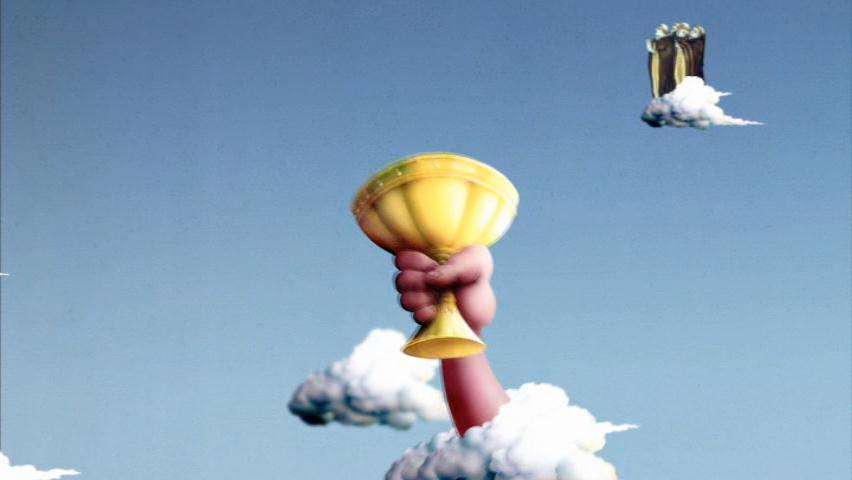
\includegraphics[width=0.8\textwidth]{grail.jpg}
%  \caption[Voorbeeld figuur.]{\label{fig:grail}Voorbeeld van invoegen van een figuur. Zorg altijd voor een uitgebreid bijschrift dat de figuur volledig beschrijft zonder in de tekst te moeten gaan zoeken. Vergeet ook je bronvermelding niet!}
%\end{figure}
%
%\begin{listing}
%  \begin{minted}{python}
%    import pandas as pd
%    import seaborn as sns
%
%    penguins = sns.load_dataset('penguins')
%    sns.relplot(data=penguins, x="flipper_length_mm", y="bill_length_mm", hue="species")
%  \end{minted}
%  \caption[Voorbeeld codefragment]{Voorbeeld van het invoegen van een codefragment.}
%\end{listing}
%
%\lipsum[7-20]
%
%\begin{table}
%  \centering
%  \begin{tabular}{lcr}
%    \toprule
%    \textbf{Kolom 1} & \textbf{Kolom 2} & \textbf{Kolom 3} \\
%    $\alpha$         & $\beta$          & $\gamma$         \\
%    \midrule
%    A                & 10.230           & a                \\
%    B                & 45.678           & b                \\
%    C                & 99.987           & c                \\
%    \bottomrule
%  \end{tabular}
%  \caption[Voorbeeld tabel]{\label{tab:example}Voorbeeld van een tabel.}
%\end{table}


%%=============================================================================
%% Methodologie
%%=============================================================================

\chapter{\IfLanguageName{dutch}{Methodologie}{Methodology}}%
\label{ch:methodologie}

%% TODO: In dit hoofstuk geef je een korte toelichting over hoe je te werk bent
%% gegaan. Verdeel je onderzoek in grote fasen, en licht in elke fase toe wat
%% de doelstelling was, welke deliverables daar uit gekomen zijn, en welke
%% onderzoeksmethoden je daarbij toegepast hebt. Verantwoord waarom je
%% op deze manier te werk gegaan bent.
%% 
%% Voorbeelden van zulke fasen zijn: literatuurstudie, opstellen van een
%% requirements-analyse, opstellen long-list (bij vergelijkende studie),
%% selectie van geschikte tools (bij vergelijkende studie, "short-list"),
%% opzetten testopstelling/PoC, uitvoeren testen en verzamelen
%% van resultaten, analyse van resultaten, ...
%%
%% !!!!! LET OP !!!!!
%%
%% Het is uitdrukkelijk NIET de bedoeling dat je het grootste deel van de corpus
%% van je bachelorproef in dit hoofstuk verwerkt! Dit hoofdstuk is eerder een
%% kort overzicht van je plan van aanpak.
%%
%% Maak voor elke fase (behalve het literatuuronderzoek) een NIEUW HOOFDSTUK aan
%% en geef het een gepaste titel.

Om de onderzoeksvraag te beantwoorden, wordt een Proof-of-Concept (PoC) ontwikkeld. Dit proces verloopt in verschillende fases, die fungeren als mijlpalen om de voortgang te bewaken en te bepalen of we op schema liggen.


\begin{enumerate}
    \item \textbf{Ontdekken van de geschikte \acrshort{LLM}}: In de eerste fase gaan we op zoek naar de juiste \acrshort{LLM}. De meeste \acrshort{LLM}'s bieden ondersteuning voor het Engels, maar wij willen vooral ondersteuning aanbieden voor het Nederlands. Daarom zoeken we een model dat vloeiend is in het Nederlands. Om dit te onderzoeken, maken we gebruik van \emph{GPT4All}.
    
    GPT4All is een tool die het mogelijk maakt om \acrshort{LLM}'s lokaal te gebruiken op een dagelijkse computer. Hierdoor is het niet langer nodig om gebruik te maken van cloudinfrastructuren of gespecialiseerde hardware om met \acrshort{LLM}'s te werken \autocite{NST2024}. De beschikbare \acrshort{LLM}'s zijn te vinden op het platform \emph{Hugging Face}. Bovendien beschikt GPT4All over een functie genaamd \emph{LocalDocs}. Met LocalDocs kunnen persoonlijke bestanden worden gebruikt als extra context voor de \acrshort{LLM}, indien relevant. Dit is zeer vergelijkbaar met RAG.
    
    Om het juiste model te kiezen, wordt elk kandidaat-model getest met een reeks vragen, waarvan de antwoorden worden vergeleken met de verwachte antwoorden. De vragen omvatten zowel algemene onderwerpen als onderwerpen gerelateerd aan de inhoud van de LocalDocs. Deze tests bieden ook de mogelijkheid om prompt-engineering toe te passen en te evalueren welk model de beste antwoorden genereert binnen de beperkingen van de prompt.
    
    Deze fase wordt als succesvol beschouwd wanneer het model met de beste prestaties is geïdentificeerd. 
    
    \textbf{Ingeschatte duurtijd}: één week en half
    
    \item \textbf{Opzetten van het PoC lokaal}: In de tweede fase wordt een zogenoemde RAG-pijplijn aangemaakt. De pijplijn bestaat uit de volgende componenten: 
    \begin{itemize} 
        \item \textbf{Source Extractor}: Deze component voert twee taken uit. De eerste taak is het opschonen van de invoerbestanden. De tweede taak is het creëren van de brokken. Deze brokken worden vervolgens doorgegeven aan de Embedder. 
               
        Om de correcte werking van dit onderdeel te testen, wordt de uitvoer van het opschoonproces van de invoerbestanden geanalyseerd, evenals de gegenereerde brokken om de correcte verdelingsstrategie voor de brokken te vinden. 
        \item \textbf{Embedder}: De Embedder is verantwoordelijk voor het omzetten van de brokken naar embeddings. Deze embeddings wordt daarna doorgegeven aan de datastore. Daarnaast zet de Embedder de invoer van de gebruiker om in een embedding om de relevante brokken te kunnen ophalen. 
        
        Hierbij moeten we bijzondere aandacht besteden aan het vinden van een Nederlandstalige embedder, aangezien embedders worden getraind op specifieke talen.

        Dit onderdeel wordt als voltooid beschouwd wanneer de embeddings correct worden gegenereerd en succesvol in de datastore worden opgeslagen
        \item \textbf{Datastore}: Binnen de datastore worden de embeddings opgeslagen. De datastore is een vector-databank die het mogelijk maakt om relevante brokken op te zoeken, gegeven de ge-embedded invoer. De relevante brokken worden vervolgens doorgegeven aan de Conversation Manager. 
        \item \textbf{Conversation Manager}: De Conversation Manager bestaat uit de eigenlijke \acrshort{LLM}, de Moderation API en een aantal voorgemaakte prompts. Deze voorgemaakte prompts dienen om de context te verrijken met de brokken en om de \acrshort{LLM} te laten reageren zoals gewenst. De prompts bevatten aanwijzingen over hoe onverwachte interacties opgelost moeten worden. Deze prompts werden gedeeltelijk in de vorige fase aangemaakt en hier verder uitgewerkt. 
        
        Deze component wordt als voltooid beschouwd wanneer de gegenereerde antwoorden daadwerkelijk gebaseerd zijn op de informatie die is opgeslagen in de datastore. Dit bevestigt dat de relevante databrokken correct worden opgehaald en gebruikt.
    \end{itemize}
    
    Om dit allemaal op te zetten, wordt LangChain gebruikt. LangChain fungeert als een framework dat het mogelijk maakt om \acrshort{LLM}'s te integreren binnen een applicatie. Binnen LangChain bestaat ook de mogelijkheid om gebruik te maken van GPT4All. Hierdoor blijft het gebruik van cloudinfrastructuren en gespecialiseerde hardware overbodig.
    
    Voor de Datastore maken we gebruik van \emph{Chroma}, een vector-databank waarmee embeddings kunnen worden opgeslagen en vergelijkbare embeddings kunnen worden opgehaald. We kiezen voor een expliciete vector-databank in plaats van LocalDocs, omdat LocalDocs alleen kunnen worden ingeschakeld via de GUI van GPT4All. Aangezien we Eureka op een server willen uitrollen, kunnen we niet vertrouwen op een GUI.
    
    Er wordt pas overgeschakeld naar het volgende onderdeel van de pijplijn wanneer de huidige component als voltooid wordt beschouwd. Zo niet, dan wordt de huidige component verder geoptimaliseerd en aangepast totdat deze correct functioneert.
    
    \textbf{Ingeschatte duurtijd}: vier weken (één week per component van de pijplijn)
    
    \item \textbf{Testen van het PoC}: Het PoC zal worden getest op vakken die worden gegeven door de heer Van Vreckem. Deze vakken zijn \emph{Data Science \& AI}, \emph{Infrastructure Automation} en \emph{Linux for Data Scientists}.
    
    De gebruikte bestanden zijn PDF-bestanden van slides, opdrachten en studiefiches. Een reeks vragen zal aan de \acrshort{LLM} worden gesteld, waarna de specialist die de docenten vertegenwoordigt (dhr. Van Vreckem) en de persoon die de studenten vertegenwoordigt de antwoorden van het model zullen beoordelen.
    
    De antwoorden moeten voldoen aan de verwachtingen van de verschillende stakeholders:
    
    \begin{itemize} 
        \item \textbf{Student}:
        \begin{enumerate} 
            \item Als student wil ik dat de gegenereerde antwoorden inhoudelijk aansluiten bij de gestelde vragen.
            \item Als student wil ik dat de antwoorden correcte informatie bevatten. 
            \item Als student wil ik dat, indien de antwoord niet gekend is, er verwijst wordt naar mogelijke pistes om een antwoord te bekomen. Echter, wil ik geen valse informatie ondervinden.
        \end{enumerate}
        \item \textbf{Docent}:
        \begin{enumerate} 
            \item Als docent wil ik dat de gegenereerde antwoorden correcte informatie bevatten voor de studenten.
            \item Als docent wil ik dat Eureka naar hulpzame bronnen verwijst zodat de student mogelijke verdere vragen zelf kan beantwoorden. 
            \item Als docent wil ik gemakkelijk mijn bronnen kunnen wijzigingen indien er aanpassingen zijn.
            \item Als docent wil ik dat de gegenereerde antwoorden passend en professioneel zijn, zonder ongepaste inhoud.
        \end{enumerate}    
    \end{itemize}
    
    Aangezien de RAG-pijplijn uit verschillende componenten bestaat, zal de test verschillende keren herhaald worden met verschillende instellingen van de pijplijn. De elementen die telkens worden gewijzigd, zijn de strategie van de brokverdeling, het type Embedder en de gebruikte \acrshort{LLM}. Dit heeft als doel de optimale instellingen te achterhalen. 
    
    Door deze evaluatiestrategie wordt verzekerd dat Eureka voldoet aan de gestelde eisen en als een betrouwbare en bruikbare tool kan fungeren voor studenten en docenten.
    
    \textbf{Ingeschatte duurtijd}: drie tot vier weken, loopt parallel met het opzetten van het PoC.
    
    \item \textbf{Uitplooien van het PoC op een server}: Zodra een overtuigende configuratie is gevonden, wordt het PoC op een server uitgerold, zodat het toegankelijk is via een REST API. Er wordt een server van het VIC hiervoor benut
\end{enumerate}



% Voeg hier je eigen hoofdstukken toe die de ``corpus'' van je bachelorproef
% vormen. De structuur en titels hangen af van je eigen onderzoek. Je kan bv.
% elke fase in je onderzoek in een apart hoofdstuk bespreken.

%\input{...}
%\input{...}
%...

%%=============================================================================
%% Conclusie
%%=============================================================================

\chapter{Conclusie}%
\label{ch:conclusie}

% TODO: Trek een duidelijke conclusie, in de vorm van een antwoord op de
% onderzoeksvra(a)g(en). Wat was jouw bijdrage aan het onderzoeksdomein en
% hoe biedt dit meerwaarde aan het vakgebied/doelgroep? 
% Reflecteer kritisch over het resultaat. In Engelse teksten wordt deze sectie
% ``Discussion'' genoemd. Had je deze uitkomst verwacht? Zijn er zaken die nog
% niet duidelijk zijn?
% Heeft het onderzoek geleid tot nieuwe vragen die uitnodigen tot verder 
%onderzoek?

\lipsum[76-80]



%---------- Bijlagen -----------------------------------------------------------

\appendix

\chapter{Onderzoeksvoorstel}

Het onderwerp van deze bachelorproef is gebaseerd op een onderzoeksvoorstel dat vooraf werd beoordeeld door de promotor. Dat voorstel is opgenomen in deze bijlage.

%% TODO: 
%\section*{Samenvatting}

% Kopieer en plak hier de samenvatting (abstract) van je onderzoeksvoorstel.

% Verwijzing naar het bestand met de inhoud van het onderzoeksvoorstel
%---------- Inleiding ---------------------------------------------------------

% TODO: Is dit voorstel gebaseerd op een paper van Research Methods die je
% vorig jaar hebt ingediend? Heb je daarbij eventueel samengewerkt met een
% andere student?
% Zo ja, haal dan de tekst hieronder uit commentaar en pas aan.

%\paragraph{Opmerking}

% Dit voorstel is gebaseerd op het onderzoeksvoorstel dat werd geschreven in het
% kader van het vak Research Methods dat ik (vorig/dit) academiejaar heb
% uitgewerkt (met medesturent VOORNAAM NAAM als mede-auteur).
% 

\section{Inleiding}%
\label{sec:inleiding}

Bij het opnemen van een vak worden studenten aan de HOGENT tijdens het semester vaak geconfronteerd met een grote hoeveelheid informatie: lesmodaliteiten, taken, deadlines, en kennismaking met de benodigde software, om enkele voorbeelden te noemen. Gedurende het semester ontstaan er regelmatig vragen bij studenten, die zij proberen te beantwoorden door de beschikbare materialen te raadplegen of door hun vragen aan medestudenten voor te leggen. Toch blijken deze informatiebronnen niet altijd voldoende---vanwege onduidelijkheden of tegenstrijdigheden---zoals blijkt uit het aantal studenten dat alsnog bij de docent aanklopt. Dit is echter niet praktisch; als een docent tien keer dezelfde vraag ontvangt, moet hij of zij die vraag ook tien keer beantwoorden. Bovendien is er geen garantie dat een student zijn of haar antwoord dezelfde dag nog ontvangt. Deze uitwisseling is dan ook een frustrerend en tijdrovend proces voor beide partijen. Er bestaat dus behoefte aan een middel dat enerzijds de werkdruk van docenten verlicht door antwoorden te geven dat op veelgestelde vragen van studenten en anderzijds deze antwoorden on demand levert. 

Deze paper heeft als doel om een toegepast onderzoek te motiveren naar Eureka, een virtuele assistent die studenten en docenten van de HOGENT ondersteunt bij het beantwoorden van vakgerelateerde vragen. In dit onderzoek wordt de haalbaarheid van een dergelijk hulpmiddel onderzocht en wordt een proof-of-concept (POC) ontwikkeld. Het POC wordt als succesvol beschouwd als minstens de volgende vragen kunnen worden beantwoord: 

\begin{itemize}
    \item Levert Eukera relevante antwoorden ? 
    \item Kan Eureka onverwachte interacties, zoals beledigingen, aan ?
    \item Hoe kan hallucinatie vermeden worden ? 
\end{itemize}

Bovendien moet de achterliggende oplossing minstens de volgende vragen kunnen beantwoorden: 

\begin{itemize} 
    \item Kan de kennis van Eureka op een eenvoudige manier worden uitgebreid of gewijzigd, zodat ook docenten met beperkte technische kennis ermee kunnen werken?
    \item Kan Eureka worden geïmplementeerd met beperkte financiële en computationele middelen?
    \item Is Eureka uitrolbaar op een server?
\end{itemize}

%---------- Stand van zaken ---------------------------------------------------

\section{Literatuurstudie}%
\label{sec:literatuurstudie}

\subsection{Stand van zaken}

Om informatie te verkrijgen, onderscheiden veel studenten twee belangrijke informatiebronnen: bronnen afkomstig van de hogeschool en informatie uitgewisseld door studenten zelf.

Vanuit de hogeschool worden verschillende bro\-nnen van informatie aangeboden waarop studenten en docenten antwoorden kunnen vinden op hun vragen. Ten eerste zijn er de inleidende slides van het vak. Hierin is informatie te vinden over eventueel aan te schaffen materialen, mogelijke softwarevereisten, deadlines en de organisatie van het vak. Verder zijn er de studiefiches beschikbaar, die algemene informatie bevatten zoals de studielast, de leerresultaten en de evaluatievorm. Bij sommige vakken worden ook aanvullende bestanden verstrekt die studenten begeleiden bij bepaalde onderwerpen en vaak voorkomende problemen of vragen behandelen. Tot slot is bij sommige vakken ook een forum beschikbaar. Dit forum dient als centrale plaats om vragen te stellen, waarbij de antwoorden zichtbaar zijn voor alle studenten.

Daarnaast maken veel mensen gebruik van sociale media om informatie over specifieke onderwerpen uit te wisselen, en studenten vormen hierop geen uitzondering. Sociale media wordt ingezet om met andere studenten over de vakinhoud te communiceren en zo nieuwe kennis op te doen. Deze veronderstelling is ook bevestigd in andere onderzoeken. \textcite{M.Talaue2018} en \textcite{Bal2017} interviewden verschillende studenten over hun gebruik van sociale media, waaruit blijkt dat een groot deel van hen sociale media gebruikt om vakken hun inhoud te bespreken. Aan de HOGENT is dit eveneens het geval. Naast hun persoonlijke profielen op andere media, komen studenten samen op een \emph{Discord}-server. Deze server is onderverdeeld in verschillende kanalen, waarbij elk kanaal een specifiek vak vertegenwoordigt. Studenten bespreken in deze kanalen alles wat met het desbetreffende vak te maken heeft en stellen er hun vragen. Aangezien deze server door studenten wordt beheerd en docenten er geen toegang toe hebben, omdat het geen officieel kanaal van HOGENT is, bestaat het risico dat er foutieve informatie wordt uitgewisseld. 

Zoals blijkt, is informatie verspreid over een verscheidenheid aan media. Informatie vinden kan daarom enige moeite kosten, en de kans op onduidelijkheden of tegenstrijdige informatie is aanzienlijk. In het geval van problemen is het laatste redmiddel voor studenten om contact op te nemen met de docent. De positie van docenten stelt hen in staat om onduidelijkheid op te helderen, maar zij beschikken niet altijd over de tijd hiervoor. Bovendien kan het herhaaldelijk beantwoorden van dezelfde vragen frustrerend zijn.

We concluderen daarom dat er behoefte is aan een middel dat het zoekproces intuïtiever maakt en de belasting voor alle betrokken partijen verlicht. Wij stellen hiervoor een chatbot in de vorm van een virtuele assistent voor en zullen deze oplossing verder onderzoeken.


\subsection{Evolutie van chatbots}
\label{sec:chatbots}

In de jaren zestig begon men met de eerste onderzoeken naar communicatie tussen computers en mensen. De onderzoekers hadden niet de intentie om grote doorbraken in het veld te realiseren, maar wilden enkel experimenteren met de grens tussen mens en machine \autocite{Dibitonto2018, AbuShawar2007}. Een van deze experimenten was \emph{ELIZA} \autocite{Weizenbaum1966}. ELIZA was ''een computerprogramma [...] dat bepaalde natuurlijke taalgesprekken tussen mens en computer mogelijk maakte''. Het werd ontwikkeld voor de IBM 7094 en geschreven in MAD-SLIP \autocite{Weizenbaum1966}. De werking van ELIZA kan grofweg als volgt worden samengevat: gegeven een invoerzin, werden vooraf gedefinieerde sleutelwoorden gezocht. Eens deze sleutelwoorden gevonden werden, werd het uiteindelijke antwoord gegenereerd door gebruik te maken van reconstructieregels. 

Naargelang de onderzoek naar chatbots vorderde, werden betere architecturen bedacht maar de kern bleef onveranderd: pattern-matching-algortimen die regels toepasten met als doel de interactie zo natuurlijk mogelijk te laten aanvoelen \autocite{AbuShawar2007}. Hoewel de toepassing van chatbots als virtuele assistenten of informatieopzoeksystemen destijds als succesvol werd beschouwd \autocite{AbuShawar2007}, is het niet moeilijk voor te stellen hoe vatbaar deze technologie is voor fouten en rigiditeit. Wanneer een bepaalde casus niet wordt gedekt door een regel of de regels onvoldoende doordacht zijn, presteert de chatbot slecht, waardoor de interactie wordt belemmerd. 

Dankzij de toenemende rekenkracht van de afgelopen jaren en de groeiende interesse in het domein van artificiële intelligentie, zien we een nieuwe generatie chatbots ontstaan. De werking van deze chatbots maakt het mogelijk om af te stappen van het pattern-matching-paradigma. Deze chatbots maken namelijk gebruik van doorbraken in \emph{Natural Language Processing} (NLP) en zijn gebaseerd op \emph{Large Language Models} (LLM's) (zie \ref{sec:llms}). Dergelijke chatbots worden al in verschillende domeinen gebruikt met overtuigende resultaten \autocite{Dell’Acqua2023, Wang2024, Azam2024}

\subsection{Large Language Models}
\label{sec:llms}

Sinds eind 2022 heeft vrijwel iedereen minstens één keer gehoord van \emph{ChatGPT}. Een analyse van de populariteit van deze term via \emph{Google Trends} laat zien dat de interesse in \emph{ChatGPT} voortdurend toeneemt. Een doorbraak in artificiële intelligentie heeft Large Language Models en, in bredere zin, Natural Language Processing in de schijnwerpers gezet. NLP kan worden gedefinieerd als ''de tak van Artificiële Intelligentie die computers helpt menselijke taal te begrijpen, interpreteren en manipuleren'' \autocite{Zohuri2022}. Het omvat een reeks technieken die het mogelijk maken voor computers om op een natuurlijke manier te communiceren met mensen. LLM's daarentegen zijn intelligente systemen die, door gebruik te maken van NLP-technieken, in staat zijn om tekst te verwerken en te genereren met samenhangende communicatie. Hoewel LLM's zeer populair zijn vandaag, is hun werking voor de meerderheid van mensen nog magie. Zodat de lezer een idee kan krijgen van wat er allemaal verbogen staat achter een LLM, geven we hier een bondig samenvatting dat gebaseerd is op \textcite{Naveed2023}.

Eem LLM is een zeer diepe kunstmatige neurale netwerken dat rust op de \emph{transformer} architectuur (geïntroduceerd door \textcite{Vaswani2017}). Elke moderne LLM heeft volgende basiscomponenten: 
\begin{itemize} 
    \item \textbf{Tokenisatie}: Dit is een pre-processing stap dat training voorgaat. Hier, wordt de invoer onderverdeelt in tokens. Een token kan een character, stuk woord, symbool of woord zijn afhankelijk van de tokenisatie-techniek dat gebruikt wordt.
    \item \textbf{Aandacht}: Deze component wijst gewichten toe aan de input tokens zodat de model meer aandacht richt aan de belangrijkste tokens.
    \item \textbf{Positionele encodering}: Hier wordt informatie toegevoegd met betrekking tot de posities van de tokens. Dit component werkt heel nauw samen met de aandacht zodat de model de invoer begrijpt. Anders uitgedrukt, wordt via aandacht de belangrijkste toekens geïdentificieert en via positionele encodering wordt de volgorde en context van deze tokens verstaan.
    \item \textbf{Activatiefunctie}: Deze functies laten toe de model om niet-lineaire relaties aan te leren, wat cruciaal is om met taal aan de slag te gaan.
\end{itemize}

De training van de LLM gebeurt volgens \textcite{Bach2024} in drie fases:
\begin{enumerate} 
    \item \textbf{Self-supervised learning}: In deze stap moet de LLM, gegeven een zin met een ontbrekend woord (of woorden), een lijst genereren van mogelijke woorden die zouden kunnen passen. Deze lijst is gerangschikt op basis van waarschijnlijkheid. Het doel van deze fase is dat het model de eigenschappen van de taal leert begrijpen, evenals de specifieke kenmerken van het datadomein.
    \item \textbf{Supervised learning}: Hier wordt het model getrained om taken uit te voeren. Voorbeelden van dergelijke taken zijn het genereren van code, het samenvatten van teksten en het beantwoorden van specifieke vragen, om er maar enkele te noemen. Het doel van deze fase is ervoor te zorgen dat het model daadwerkelijk nuttige taken kan uitvoeren in plaats van simpelweg woorden te raden.
    \item \textbf{Reinforcement learning}: In deze stap worden de gewenste gedragen aan het model aangeleerd. Dit gebeurt door gewenst gedrag te belonen en ongewenst gedrag te bestraffen.
\end{enumerate}

De indrukwekkende prestaties van LLM's in een reeks van taken (\autocite{Naveed2023}) zijn te danken aan de hedendaagse rekenkracht, de e\-nor\-me hoeveelheid beschikbare data (voortgebracht door sociale media en het \emph{Internet of Things}), en de groeiende interesse in dit domein \autocite{Zohuri2022, Naveed2023}. Hierdoor zijn LLM's uitermate geschikt als basis voor de ontwikkeling van Eureka. 

\subsection{Ontwerp}

\subsubsection{Specialiseren van LLM's}

Het doel van dit onderzoek is om een chatbot te implementeren, gebaseerd op een LLM, die vragen over vakken \textbf{gegeven aan de HOGENT} kan beantwoorden. Dit betekent dat onze LLM gespecialiseerde kennis moet hebben, in plaats van de algemene kennis die door bekende LLM's wordt gebruikt. Om een LLM te specialiseren, zijn er drie benaderingen mogelijk: zelf een LLM ontwerpen, een bestaande LLM \emph{fine-tunen}, of de kennis van een LLM uitbreiden met behulp van \emph{context-injectie}

De eerste benadering houdt in dat we zelf een LLM vanaf nul bouwen en trainen op door ons aangeleverde data. Dit is echter niet haalbaar vanwege de aanzienlijke middelen, expertise \autocite{Naveed2023} en tijd die hiervoor nodig zijn. \textcite{Fourrier2024} somt verschillende open-source LLM's op, waarvan de meeste meer dan één miljard parameters bevatten. Het is duidelijk dat het trainen van een model met één miljard parameters veel tijd kost en dat het ontwikkelen van een dergelijk model ook een hoog niveau van expertise vereist.

Bij de tweede benadering wordt een bestaande LLM gebruikt, waarbij de gewichten worden aangepast om de LLM te specialiseren voor het specifieke doel waarvoor we deze nodig hebben. Zo hebben \textcite{Azam2024} PharmaLLM ontwikkeld, een chatbot die vragen over medicijnen kan beantwoorden. Dit model werd ontworpen door het Llama 2-model te fine-tunen met behulp van \emph{Low-Rank Adaptation} (LoRA). Met LoRA worden alleen de meest impactvolle gewichten aangepast om het model te specialiseren, waardoor het niet nodig is om alle gewichten van het model volledig te hertrainen. Enkel een subset van de gewichten wordt gewijzigd, wat aanzienlijk minder middelen vereist dan de eerste benadering. Hierdoor wordt de specialisatie haalbaar zonder de volledige parameterstructuur te hertrainen.

Hoewel de tweede benadering haalbaarder lijkt, blijven de vereiste middelen aanzienlijk. Zo beschrijven \textcite{Chiang2023} de ontwikkeling van een LLM waarbij zij het model hebben gefinetuned. Om aan hun criteria te voldoen, maakten ze gebruik van acht \emph{A100}-GPU's, waarbij elke trainingssessie meer dan 300 dollar kostte. Bovendien is er, om de juiste fine-tuningtechniek te kiezen - LoRA is niet de enige techniek - en het model optimaal te fine-tunen, opniew expertise vereist.

De laatste benadering maakt gebruikt van een techniek die we context-injectie gaan noemen. Elk LLM beschikt over een \emph{contextvenster}. In dit venster kan extra context worden toegevoegd die het LLM in rekening neemt bij het genereren van zijn antwoord. Het doel van context-injectie is om relevante informatie met betrekking tot de gestelde vraag in het venster te plaatsen. De informatie over de vakken wordt opgeslagen in een databank. Afhankelijk van de gestelde vraag halen we alleen de relevante informatie op. Met deze benadering kunnen we een bestaande LLM gebruiken zonder een trainingsfase, wat resulteert in lagere middelen en expertise die gemakkelijker toegankelijk is. Context-injectie samen met de data vanuit een databank ophalen is wat men \emph{Retrieval-Augmented-Generation} (RAG) noemt. Deze techniek wordt al succesvol toegepast in verschillende domeinen. We nodigen de lezer uit om \textcite{Wang2024} te raadplegen voor een voorbeeld van ee chatbot die gebruikmaakt van RAG en een vergelijkbaar doel nastreeft als het onze. 

De laatste benadering is de meest veelbelovende met betrekking tot onze doelstellingen. Ze vraagt minder middelen en vereist geen vakexpertise om te benutten. We onderzoeken deze piste verder.

\subsubsection{Retrieval-augmented-generation}

In 2020 maakten \textcite{Lewis2020} de volgende vaststelling: LLM's zijn zeer geschikt om diepe inzichten te verkrijgen uit de data waarop ze getraind zijn. Hierdoor hebben ze geen externe \emph{knowledge bases} nodig om vragen te beantwoorden; hun vergaarde kennis fungeert als een impliciete knowledge base. Echter brengt dit enkele uitdagingen met zich mee. Ten eerste is het moeilijk om bestaande kennis te actualiseren zonder het leerproces volledig opnieuw te starten. Dit vormt een tijdrovend proces wanneer frequente updates noodzakelijk zijn. Daarnaast hebben LLM's moeite om vragen te beantwoorden over gebeurtenissen die zich hebben voorgedaan na hun laatste trainingssessie, aangezien ze deze kennis niet bezitten. Dit kan leiden tot hallucinaties \autocite{Gao2023}.

Om deze beperkingen aan te pakken, introduceerden de auteurs een nieuwe techniek genaamd Retrieval-Augmented Generation (RAG). Bij deze techniek wordt een vraag beantwoord door aanvullende kennis op te halen uit externe bronnen en deze te gebruiken om een antwoord te genereren. Zoals \textcite{Lewis2020} het omschrijven: ''De invoersequentie $x$ wordt gebruikt om tekstdocumenten $z$ op te halen, die vervolgens dienen als aanvullende context bij het genereren van de doelsequentie $y$''.

Alle RAG-systemen bestaan uit drie belangrijke stappen \autocite{Gao2023}:  

\begin{enumerate} 
    \item \textbf{Indexing}: Hier wordt ruwe data uit verschillende formaten (bijvoorbeeld PDF, HTML, DOCX) opgehaald. Vervolgens wordt deze data geconverteerd naar tekst en opgeschoond. Belangrijk hierbij is dat de tekst wordt opgedeeld in brokken. De reden hiervoor is dat het contextvenster van LLM's een beperkte grootte heeft, waardoor het beter is om alleen de relevante brok door te geven in plaats van het gehele document, waarbij het risico bestaat dat niet alles past. Bovendien is uit onderzoek gebleken dat LLM's meer aandacht besteden aan het begin en einde van het contextvenster en minder aan het midden. Dit fenomeen staat bekend als het \emph{lost in the middle}-fenomeen \autocite{Databricks}. Daarom is het beter om kleinere contexten door te geven dan grote, zodat de aandacht van de LLM behouden blijft. Uiteindelijk, worden de brokken opgeslaan in een vector-databank door gebruik te gaan maken van \emph{embedding} encodering.
    \item \textbf{Retrieval}: In deze fase wordt de gebruikersinvoer omgezet in een vectorvoorstelling met behulp van dezelfde encodering als in de vorige stap. Op basis van deze vectorvoorstelling worden de relevante brokken opgehaald. Relevantie in deze context verwijst naar de brokken die een verband hebben met de gestelde vraag. Dit verband wordt bepaald door middel van vectorvergelijkingen. De opgehaalde brokken worden vervolgens gebruikt om het contextvenster te verrijken.
    \item \textbf{Generation}: Tot slot wordt het finale antwoord gegenereerd. Merk op dat de LLM voornamelijk wordt gebruikt voor haar taalcapaciteiten bij het formuleren van het antwoord. Het grootste deel van het werk wordt echter uitgevoerd in de twee voorgaande fases.
\end{enumerate}

\subsubsection{Valkuilen}

Bij het ontwerpen van Eureka zijn er twee belangrijke valkuilen die bijzondere aandacht vereisen: \textbf{onverwachte interacties} en \textbf{hallucinaties}.

Tijdens de ontwikkeling van de chatbot \emph{LiSA} constateerden \textcite{Dibitonto2018} dat er een tendens bestond om LiSA te antropomorfiseren, ondanks haar beperkte complexiteit. Dit resulteerde in onverwachte reacties, zoals uitingen van dankbaarheid of het gebruik van smileys om zinnen te benadrukken. Helaas leidde dit ook tot ongepast gedrag; sommige gebruikers reageerden agressief of gaven de interactie een seksuele connotatie. Onverwachte interacties kunnen echter niet alleen voortkomen uit gebruikers, maar ook uit de chatbot zelf.

Een voorbeeld hiervan is \emph{Prompt Hacking}, een aanvalsmethode waarbij specifieke prompts worden ingevoerd met als doel de LLM gedrag te laten vertonen dat afwijkt van de oorspronkelijke bedoeling van het model \autocite{Rababah2024}. Dergelijk afwijkend gedrag kan bijvoorbeeld bestaan uit het openbaar maken van privé-informatie of het maken van beledigende opmerkingen \autocite{Naveed2023}.

Daarnaast is vastgesteld dat LLM's onderhevig kunnen zijn aan een fenomeen dat bekend staat als \emph{hallucinatie}. Hierbij genereert de LLM coherente uitvoer die echter gebaseerd is op onjuiste informatie. Dit fenomeen kan worden onderverdeeld in drie categorieën \autocite{Naveed2023}:

\begin{itemize} 
    \item \textbf{Input-conflicterende hallucinatie}: de gegenereerde output heeft weinig tot geen verband met de ingevoerde gegevens. 
    \item \textbf{Context-conflicterende hallucinatie}: de gegenereerde output is in tegenspraak met eerder gegenereerde output. 
    \item \textbf{Feit-conflicterende hallucinatie}: de output bevat onjuiste informatie over algemeen bekende feiten (bijvoorbeeld: ''Parijs is de hoofdstad van Pakistan''). 
\end{itemize}

Hallucinaties dienen strikt vermeden te worden bij het ontwerpen van Eureka, aangezien ze het risico met zich meebrengen om meer verwarring te zaaien in plaats van duidelijkheid te bieden.

\subsection{Besluit}

Uit de literatuurstudie blijkt dat een chatbot een geschikte oplossing biedt om een centrale plaats te creëren waar studenten en docenten op een interactieve manier hun vragen kunnen stellen en on-demand een antwoord kunnen ontvangen.

Chatbots zijn een technologie die al geruime tijd bestaat en oorspronkelijk voornamelijk gebaseerd was op patroonherkenning. Met de vooruitgang in NLP en, meer specifiek, in LLM's, kunnen we nu flexibelere chatbots ontwikkelen die niet langer afhankelijk zijn van strikt gedefinieerde regels. Het zelf ontwikkelen van een LLM valt echter buiten de scope van dit onderzoek en overschrijdt de beschikbare middelen. Daarom is besloten om een bestaande LLM te gebruiken.

Aangezien bestaande LLM's vaak worden geleverd met vooraf vergaarde kennis, en we niet beschikken over de expertise om deze kennis direct te bewerken, is het noodzakelijk om de context van de LLM uit te breiden met externe bronnen. Om dit te realiseren, zal gebruik worden gemaakt van RAG, een techniek die specifiek is ontworpen voor dit doel.

Bij het ontwerp van Eureka zal er bovendien aandacht besteed moeten worden aan de valkuilen die voortkomen uit de menselijke natuur. Eureka moet voorbereid zijn op onverwachte interacties en situaties.

%---------- Methodologie ------------------------------------------------------
\section{Methodologie}%
\label{sec:methodologie}

Om de onderzoeksvraag te beantwoorden, wordt een Proof-of-Concept (PoC) ontwikkeld. Dit proces verloopt in verschillende fases, die fungeren als mijlpalen om de voortgang te bewaken en te bepalen of we op schema liggen.


\begin{enumerate}
    \item \textbf{Ontdekken van de geschikte LLM}: In de eerste fase gaan we op zoek naar de juiste LLM. De meeste LLM's bieden ondersteuning voor het Engels, maar wij willen vooral ondersteuning aanbieden voor het Nederlands. Daarom zoeken we een model dat vloeiend is in het Nederlands. Om dit te onderzoeken, maken we gebruik van \emph{GPT4All}.

    GPT4All is een tool die het mogelijk maakt om LLM's lokaal te gebruiken op een dagelijkse computer. Hierdoor is het niet langer nodig om gebruik te maken van cloudinfrastructuren of gespecialiseerde hardware om met LLM's te werken \autocite{NST2024}. De beschikbare LLM's zijn te vinden op het platform \emph{Hugging Face}. Bovendien beschikt GPT4All over een functie genaamd \emph{LocalDocs}. Met LocalDocs kunnen persoonlijke bestanden worden gebruikt als extra context voor de LLM, indien relevant. Dit is zeer vergelijkbaar met RAG.

    Om het juiste model te kiezen, wordt elk kandidaat-model getest met een reeks vragen, waarvan de antwoorden worden vergeleken met de verwachte antwoorden. De vragen omvatten zowel algemene onderwerpen als onderwerpen gerelateerd aan de inhoud van de LocalDocs. Deze tests bieden ook de mogelijkheid om prompt-engineering toe te passen en te evalueren welk model de beste antwoorden genereert binnen de beperkingen van de prompt.

    Deze fase wordt als succesvol beschouwd wanneer het model met de beste prestaties is geïdentificeerd. 

    \textbf{Ingeschatte duurtijd}: één week en half
    
    \item \textbf{Opzetten van het PoC lokaal}: In de tweede fase wordt een zogenoemde RAG-pijplijn aangemaakt. De pijplijn bestaat uit de volgende componenten: 
    \begin{itemize} 
        \item \textbf{Source Extractor}: Deze component voert twee taken uit. De eerste taak is het opschonen van de invoerbestanden. De tweede taak is het creëren van de brokken. Deze brokken worden vervolgens doorgegeven aan de Embedder. 
       
        Om de correcte werking van dit onderdeel te testen, wordt de uitvoer van het opschoonproces van de invoerbestanden geanalyseerd, evenals de gegenereerde brokken. 
        \item \textbf{Embedder}: De Embedder is verantwoordelijk voor het omzetten van de brokken naar embeddings. Een embedding kan worden gezien als een vectorvoorstelling van de brokken. Deze vectorvoorstelling wordt daarna doorgegeven aan de datastore. Daarnaast zet de Embedder de invoer van de gebruiker om in een embedding om de relevante brokken te kunnen ophalen. 
       
        Dit onderdeel wordt als voltooid beschouwd wanneer de embeddings correct worden gegenereerd en succesvol in de datastore worden opgeslagen
        \item \textbf{Datastore}: Binnen de datastore worden de embeddings opgeslagen. De datastore is een vector-databank die het mogelijk maakt om relevante brokken op te zoeken, gegeven de ge-embedded invoer. De relevante brokken worden vervolgens doorgegeven aan de Conversation Manager. 
        \item \textbf{Conversation Manager}: De Conversation Manager bestaat uit de eigenlijke LLM en een aantal voorgemaakte prompts. Deze voorgemaakte prompts dienen om de context te verrijken met de brokken en om de LLM te laten reageren zoals gewenst. De prompts bevatten aanwijzingen over hoe onverwachte interacties opgelost moeten worden. Deze prompts werden gedeeltelijk in de vorige fase aangemaakt en hier verder uitgewerkt. 
       
        Deze component wordt als voltooid beschouwd wanneer de gegenereerde antwoorden daadwerkelijk gebaseerd zijn op de informatie die is opgeslagen in de datastore. Dit bevestigt dat de relevante databrokken correct worden opgehaald en gebruikt.
   \end{itemize}
   
    Om dit allemaal op te zetten, wordt LangChain gebruikt. LangChain fungeert als een framework dat het mogelijk maakt om LLM’s te integreren binnen een applicatie. Binnen LangChain bestaat ook de mogelijkheid om gebruik te maken van GPT4All. Hierdoor blijft het gebruik van cloudinfrastructuren en gespecialiseerde hardware overbodig.
   
    Voor de Datastore maken we gebruik van \emph{Chroma}, een vector-databank waarmee embeddings kunnen worden opgeslagen en vergelijkbare embeddings kunnen worden opgehaald. We kiezen voor een expliciete vector-databank in plaats van LocalDocs, omdat LocalDocs alleen kunnen worden ingeschakeld via de GUI van GPT4All. Aangezien we Eureka op een server willen uitrollen, kunnen we niet vertrouwen op een GUI.
   
    Er wordt pas overgeschakeld naar het volgende onderdeel van de pijplijn wanneer de huidige component als voltooid wordt beschouwd. Zo niet, dan wordt de huidige component verder geoptimaliseerd en aangepast totdat deze correct functioneert.
   
    \textbf{Ingeschatte duurtijd}: vier weken (één week per component van de pijplijn)
    
    \item \textbf{Testen van het PoC}: Het PoC zal worden getest op vakken die worden gegeven door de heer Van Vreckem. De gebruikte bestanden zijn PDF-bestanden van slides, opdrachten en studiefiches. Een reeks vragen zal aan de LLM worden gesteld, waarna de specialist (dhr. Van Vreckem) de antwoorden van het model beoordeelt. De antwoorden moeten voldoen aan de verwachtingen van de verschillende stakeholders
    
    \begin{itemize} 
        \item \textbf{Student}:
            \begin{enumerate} 
                \item Als student wil ik dat de gegenereerde antwoorden inhoudelijk aansluiten bij de gestelde vragen.
                \item Als student wil ik dat de antwoorden correcte informatie bevatten. 
                \item Als student wil ik dat, indien de antwoord niet gekend is, er verwijst wordt naar mogelijke pistes om een antwoord te bekomen. Echter, wil ik geen valse informatie ondervinden.
            \end{enumerate}
        \item \textbf{Docent}:
            \begin{enumerate} 
                \item Als docent wil ik dat de gegenereerde antwoorden correcte informatie bevatten voor de studenten.
                \item Als docent wil ik dat Eureka naar hulpzame bronnen verwijst zodat de student mogelijke verdere vragen zelf kan beantwoorden. 
                \item Als docent wil ik gemakkelijk mijn bronnen kunnen wijzigingen indien er aanpassingen zijn.
                \item Als docent wil ik dat de gegenereerde antwoorden passend en professioneel zijn, zonder ongepaste inhoud.
            \end{enumerate}    
    \end{itemize}
    
    Aangezien de RAG-pijplijn uit verschillende componenten bestaat, zal de test verschillende keren herhaald worden met verschillende instellingen van de pijplijn. De elementen die telkens worden gewijzigd, zijn de broklengte, het type Embedder en de gebruikte LLM. Dit heeft als doel de optimale instellingen te achterhalen. Het testen
    
    Door deze evaluatiestrategie wordt verzekerd dat Eureka voldoet aan de gestelde eisen en als een betrouwbare en bruikbare tool kan fungeren voor studenten en docenten.
    
    \textbf{Ingeschatte duurtijd}: drie tot vier weken, loopt parallel met het opzetten van het PoC.
    
    \item \textbf{Uitplooien van het PoC op een server}: Zodra een overtuigende configuratie is gevonden, wordt het PoC op een server uitgerold, zodat het toegankelijk is via een REST API.
\end{enumerate}


%---------- Verwachte resultaten ----------------------------------------------
\section{Verwacht resultaat, conclusie}%
\label{sec:verwachte_resultaten}

Het resultaat van dit alles is Eureka, een virtuele assistent die docenten en studenten succesvol bijstaat met hun vragen. Eureka wordt beschikbaar gesteld via een REST API. Het systeem kan onverwachte interacties afhandelen en geeft toe wanneer het iets niet weet.

Dankzij de Datastore wordt de mogelijkheid geopend om eenvoudig kennis toe te voegen of aan te passen zonder het gehele model te hoeven hertrainen. Dit maakt Eureka zeer flexibel in de dynamische omgeving van het onderwijs en toegankelijk voor gebruikers zonder dat zij experts hoeven te zijn om Eureka te onderhouden.

%%---------- Andere bijlagen --------------------------------------------------
% TODO: Voeg hier eventuele andere bijlagen toe. Bv. als je deze BP voor de
% tweede keer indient, een overzicht van de verbeteringen t.o.v. het origineel.
%\input{...}

%%---------- Backmatter, referentielijst ---------------------------------------

\backmatter{}

\setlength\bibitemsep{2pt} %% Add Some space between the bibliograpy entries
\printbibliography[heading=bibintoc]

\end{document}
